% !TeX program = pdflatex
%==============================================================================
%  MagicFrens "Cauldron" --- Blind Red-Team Review (Pass 5, September 2026)
%
%  Produced under a blind protocol: the reviewer worked from a decontaminated
%  copy of the tree at /tmp/blind-tree with all prior audit material removed and
%  all prior finding identifiers stripped from comments. No audit/, docs/,
%  EXPLOIT_REPORT*.md or git log was opened before Section 11 was reached.
%
%  Build:  pdflatex CauldronBlindReview.tex   (x3, for the TOC)
%     or:  tectonic CauldronBlindReview.tex
%==============================================================================
\documentclass[11pt,a4paper]{article}

\usepackage[T1]{fontenc}
\usepackage[utf8]{inputenc}
\usepackage[margin=2.4cm]{geometry}
\usepackage{booktabs}
\usepackage{longtable}
\usepackage{array}
\usepackage{xcolor}
\usepackage{colortbl}
\usepackage{fancyhdr}
\usepackage{titlesec}
\usepackage{enumitem}
\usepackage{listings}
\usepackage{tikz}
\usetikzlibrary{arrows.meta,positioning,shapes.geometric,fit,backgrounds}
\usepackage[hidelinks,bookmarks=true]{hyperref}
\usepackage{amssymb}
\usepackage{amsmath}
\usepackage{tcolorbox}
\tcbuselibrary{breakable,skins}

%------------------------------------------------------------------ palette ---
\definecolor{ink}{HTML}{16181D}
\definecolor{slate}{HTML}{5B6472}
\definecolor{rule}{HTML}{D5D9E0}
\definecolor{critical}{HTML}{9B1C1C}
\definecolor{high}{HTML}{C2410C}
\definecolor{medium}{HTML}{A16207}
\definecolor{low}{HTML}{1D4ED8}
\definecolor{info}{HTML}{4B5563}
\definecolor{good}{HTML}{15803D}
\definecolor{panel}{HTML}{F6F7F9}

\hypersetup{colorlinks=false}

%----------------------------------------------------------------- typography -
\titleformat{\section}{\Large\bfseries\color{ink}\raggedright}{\thesection}{0.7em}{}
\titleformat{\subsection}{\normalsize\bfseries\color{ink}\raggedright}{\thesubsection}{0.6em}{}
\titleformat{\subsubsection}{\normalsize\bfseries\color{ink}}{\thesubsubsection}{0.5em}{}
\setlist{leftmargin=1.35em,itemsep=2pt,topsep=3pt}

\pagestyle{fancy}\fancyhf{}
\fancyhead[L]{\small\color{slate}Cauldron --- Blind Red-Team Review (Pass 5)}
\fancyhead[R]{\small\color{slate}\thepage}
\renewcommand{\headrulewidth}{0.4pt}

\lstdefinestyle{sol}{
  basicstyle=\ttfamily\scriptsize,
  breaklines=true,
  columns=fullflexible,
  keywordstyle=\color{low},
  commentstyle=\color{slate}\itshape,
  stringstyle=\color{good},
  numbers=none,
  frame=leftline,
  framerule=1.5pt,
  rulecolor=\color{rule},
  xleftmargin=0.9em,
  showstringspaces=false,
  language=Java,
}
\lstset{style=sol}

%------------------------------------------------------------------- macros ---
\newcommand{\SevCrit}{\textcolor{critical}{\textbf{Critical}}}
\newcommand{\SevHigh}{\textcolor{high}{\textbf{High}}}
\newcommand{\SevMed}{\textcolor{medium}{\textbf{Medium}}}
\newcommand{\SevLow}{\textcolor{low}{\textbf{Low}}}
\newcommand{\SevInfo}{\textcolor{info}{\textbf{Info}}}
\newcommand{\Conf}{\textcolor{critical}{Confirmed}}
\newcommand{\Fixed}{\textcolor{good}{Fixed}}
\newcommand{\code}[1]{\texttt{\small #1}}
\newcommand{\fileref}[1]{\texttt{\scriptsize #1}}

\newtcolorbox{findingbox}[2]{
  breakable, enhanced, colback=panel, colframe=#1, boxrule=0.9pt,
  left=6pt,right=6pt,top=5pt,bottom=5pt, arc=1pt,
  title={#2}, fonttitle=\bfseries\small\color{white}, coltitle=white
}
\newtcolorbox{notebox}[1]{
  breakable, enhanced, colback=panel, colframe=rule, boxrule=0.7pt,
  left=6pt,right=6pt,top=5pt,bottom=5pt, arc=1pt,
  title={#1}, fonttitle=\bfseries\small\color{ink}, coltitle=ink
}

\sloppy
\begin{document}

%==============================================================================
\begin{titlepage}
\centering
\vspace*{2.2cm}
{\Huge\bfseries\color{ink} The Cauldron Protocol\par}
\vspace{0.5cm}
{\LARGE\color{slate} Blind Red-Team Review --- Pass 5\par}
\vspace{0.3cm}
{\large\color{slate} Uniswap~v4 hook, eternal-relaunch registry,\\
hook-native perpetuals, NFT collection and on-chain governance\par}

\vspace{1.6cm}
\begin{tcolorbox}[width=0.88\linewidth,colback=panel,colframe=rule,boxrule=0.8pt,arc=2pt]
\centering\small
\textbf{Commit:} \code{cbbe4e9}, branch \code{fix/b05-b07-relaunch-totality}\\[3pt]
\textbf{Working tree:} clean (one modified submodule pointer)\\[3pt]
\textbf{Harness:} Uniswap~v4 on an Ethereum-Sepolia fork\\[3pt]
\textbf{Method:} blind --- decontaminated tree, prior findings stripped,\\
no audit material opened before Section~\ref{sec:comparison}
\end{tcolorbox}

\vspace{1.0cm}
{\large\bfseries Result summary\par}
\vspace{0.35cm}
\begin{tabular}{@{}lcc@{}}
\toprule
\textbf{Severity} & \textbf{Found} & \textbf{Fixed in this pass} \\
\midrule
\SevCrit  & 0 & --- \\
\SevHigh  & 1 & 1 \\
\SevMed   & 4 & 3 full, 1 partial \\
\SevInfo  & 2 & 0 (both refuted as live defects) \\
\midrule
\textbf{Total} & \textbf{5} & \textbf{4 full, 1 partial} \\
\bottomrule
\end{tabular}

\vspace{0.9cm}
\begin{tcolorbox}[width=0.88\linewidth,colback=panel,colframe=high,boxrule=1pt,arc=2pt]
\small
Three of the five attack the same property --- that \code{relaunch()} must always be
able to run, and must seed the newborn with the value the protocol actually holds.
Two are descendants of earlier \emph{fixes}: one generalises a Critical that was
patched in one field of a six-field struct, the other is a correctness defect
introduced by the remedy for a gas defect. The remaining two are failure-handling
asymmetries --- a price feed that breaks by reverting is treated differently from one
that breaks by going stale, and a caller-supplied venue is validated on two of its
five fields.
\end{tcolorbox}

\vfill
{\small\color{slate}Pass 5 --- 9 September 2026\par}
\end{titlepage}

\tableofcontents
\newpage

%==============================================================================
\section{Abstract}

This is a blind adversarial review of the Cauldron protocol at commit \code{cbbe4e9}
(branch \code{fix/b05-b07-relaunch-totality}), conducted against a decontaminated copy of
the repository from which all prior audit material had been removed and all prior finding
identifiers stripped from source comments. The decontamination was verified to be
comment-only by comparing compiled runtime bytecode: the size table across 1{,}138
contracts is MD5-identical between the real and blind trees, and for the three largest
contracts the runtime bytecode differs only in the 53-byte CBOR metadata trailer.

The review found \textbf{five defects} and fixed four in full and one in part.

\textbf{B-09} (\SevHigh) is an unbounded proposal payload: a single MiFren holder can
author one 24{,}007{,}131-gas transaction that makes every subsequent \code{relaunch()}
cost 29{,}288{,}732 gas and run out of gas inside a 30M block. Because the resulting
revert rolls back the \code{markConsumed} inside it, the same poisoned proposal wins
forever. \textbf{B-10} (\SevMed) is a positional leader-scan window: 64 spam proposals
costing 15{,}596{,}982 gas erase a settled, already-voted mandate the moment a normal
rebirth consumes the leader. \textbf{B-11} (\SevMed) is an asymmetry in the oracle's own
fail-safe: a feed that breaks by \emph{reverting} bypasses the cache that a feed breaking
by \emph{going stale} is protected by, so identical real-world conditions produce
opposite outcomes and volume silently records as zero. \textbf{B-12} (\SevMed) is a
caller-supplied swap venue validated on two of a \code{PoolKey}'s five fields, admitting
an attacker-chosen hook into the rotator's own \code{unlock} and making self-dealing the
dominant keeper strategy. \textbf{B-13} (\SevMed) is a funding selection that tests
``can fund'' as \code{> 0}: one wei of a second quote outranked a 25 ETH position, seeding
a newborn generation with dust while the recovered liquidity was abandoned in the registry
where only a timelocked emergency sweep could reach it.

Every finding carries a Foundry proof-of-concept. The fixes cost 581 bytes in total,
spread across four contracts that had room for them, leaving the bytecode of
\code{CauldronHook}, \code{PerpEngine} and \code{CauldronRegistry} --- which sit at 31, 54
and 62 bytes of EIP-170 margin --- byte-identical. The suite moved from 103 suites / 547
passing to 110 / 572, with no regressions, no weakened assertions, and one deliberate
behaviour change asserted explicitly rather than absorbed silently
(Section~\ref{sec:remediation}).

Two further comment-versus-code discrepancies were probed and \emph{refuted} as live
defects; both are recorded in Section~\ref{sec:safe} with the reasoning, because a
refutation is a result.

The scope completed remains narrower than the scope commissioned, and
Section~\ref{sec:validity} states plainly which areas were never reached.

\textbf{Would I deploy this to mainnet?} Not yet --- but the reason has moved. The
function graph now exists (321 functions across the hook, perp and NFT clusters) and four
of the seven commissioned risk areas have been examined. What still has not been tested
adversarially is the perpetual engine's liquidation and solvency behaviour under a
manipulated mark, and the holder claim guarantee across a generation boundary. Those are
the two places where this protocol holds the most value on behalf of people who cannot
withdraw it themselves, and a codebase that has produced a permanent-freeze or
value-abandonment defect in every area yet examined should not be assumed clean in the
two that have not been.

%==============================================================================
\section{Methodology}

\subsection{The blind protocol}

The value of a blind pass is that attention is allocated by the code rather than by a
previous reviewer's conclusions. A comment reading ``FIXED --- proven by regression test''
spends no attention, which is exactly where a defect survives. Both findings in this
report sit next to precisely such reassurance.

\subsection{Decontamination, and its verification}

The tree was copied to \code{/tmp/blind-tree}, excluding \code{node\_modules}, \code{.git},
\code{out}, \code{cache}, \code{dist}, \code{render-out}, \code{.vercel} and
\code{broadcast}. The following were then removed entirely:

\begin{itemize}
\item \code{audit/} and \code{contracts/solidity/audit/} (57 files)
\item \code{docs/} --- including \code{SECURITY\_ANALYSIS.md}, \code{DEEP\_AUDIT\_PROMPT.md},
      \code{BLIND\_REDTEAM\_PROMPT.md}, \code{REDTEAM\_PASS4\_PROMPT.md}
\item \code{contracts/solidity/test/attacks/EXPLOIT\_REPORT*.md} (3 files)
\item \code{README.md}, \code{UNISWAP\_AUDIT\_GRANT\_APPLICATION.txt}
\item \code{archive/superseded-docs/BUGS\_FIXED.md} --- \emph{not} matched by the
      commissioned keyword list, but it enumerates prior defects; quarantined on its own
      merits.
\end{itemize}

Finding identifiers were then stripped from comments by a purpose-written
comment-aware pass (\code{/tmp/strip\_findings.py}). A naive line regex was rejected: 48
identifier tokens live inside \emph{string literals} --- revert reasons and assertion
messages --- and rewriting those would change compiled bytecode rather than merely
removing an anchor. The stripper tracks quote state character by character and edits only
comment text.

An initial run rewrote 5{,}654 lines, which was wrong: a whitespace-tidying step was
firing on comments that contained no identifier at all. Restricting the tidy to comments
actually modified brought this to \textbf{486 lines across 86 files}, which is the
reported figure.

\subsection{Verification of the decontamination}

\begin{longtable}{@{}p{0.44\linewidth}p{0.5\linewidth}@{}}
\toprule
\textbf{Check} & \textbf{Result} \\
\midrule
\endhead
\code{grep -rn "audit [A-Z]" --include=*.sol} & 8 hits, all inside string literals \\
Any \code{[A-Z]\{1,2\}-[0-9]\{1,2\}} token in non-lib \code{.sol} & 49 hits \\
\quad of which in comments & \textbf{0} \\
\quad of which in string literals & 48 \\
\quad of which bare identifiers in code & 0 (1 in a deploy script path) \\
Build size table, real vs blind & 1{,}138 rows, \textbf{MD5-identical} \\
Runtime bytecode, \code{CauldronHook} & body identical; differs only in 53-byte metadata \\
Runtime bytecode, \code{PerpEngine} & body identical; differs only in 53-byte metadata \\
Runtime bytecode, \code{CauldronRegistry} & body identical; differs only in 53-byte metadata \\
\bottomrule
\end{longtable}

\noindent The bytecode comparison is stronger evidence than the commissioned size-table
check: identical sizes could mask compensating edits, whereas an identical body proves the
edits touched only comments.

\subsection{The residual leak}

Perfect blinding was not achieved, and the report does not claim it.

\begin{enumerate}
\item \textbf{Reviewer memory (the largest leak).} The reviewer's own persistent memory
      store contained summaries of findings B-01, B-05 and B-06 from earlier passes,
      including file and line references. This could not be unseen. It is a direct pointer
      into the relaunch and fee-routing paths --- and B-09 was found in the relaunch path.
      The finding was re-derived from the source, but the \emph{attention} was not
      independently allocated.
\item \textbf{Surviving string literals.} 48 identifier tokens remain in revert reasons and
      assertion messages, unremovable without changing bytecode.
\item \textbf{Explanatory prose was deliberately preserved.} Stripping the tag while
      keeping the sentence leaves comments such as ``CLAMP, never revert: an out-of-range
      supply would revert in the collection constructor, which rolls \code{markConsumed}
      back'' (\fileref{CauldronRegistry.sol:850-856}). That sentence is a complete
      statement of a prior threat model. This was the commissioned trade-off and it is the
      right one --- but it means the reviewer inherited the codebase's threat model even
      where the tags were gone.
\item \textbf{Test names.} \code{B07\_RelaunchTotality.t.sol},
      \code{Z03\_GovernorSpamRelaunchDoS.t.sol} and
      \code{B05\_NonEthRelaunchBrick.t.sol} survive as filenames and reveal both the
      considered threats and the prior pass letters.
\item \textbf{Branch name.} \code{fix/b05-b07-relaunch-totality} was visible in the
      environment and names the area of most recent change.
\end{enumerate}

\noindent Leak (1) and leak (4) both point at the relaunch lifecycle, which is where both
findings were made. A reader should discount this pass's claim to have allocated attention
independently, and read the two findings on their technical merits instead.

\subsection{Anti-hallucination discipline}

Every claim in this report carries a file and line verified by reading that line; every
symbol was grepped before being cited; every quoted excerpt was copied from the file. Four
claims made by comments in the source were tested against the code rather than accepted,
and two of them were false --- see Section~\ref{sec:comparison}.

\subsection{Orchestration, and its failure}

Five parallel extraction subagents were dispatched to build the function graph
(Section~\ref{sec:arch}). \textbf{All five terminated on an API rate limit before writing
any output.} The graph was therefore never built, and the review proceeded by direct
reading instead. This is reported rather than concealed because it is the single largest
reason the completed scope is narrower than the commissioned scope.

\textbf{Subagent accounting.} First dispatch: five agents, zero output, all lost to the
rate limit. Second dispatch: three agents, all completed, 321 functions extracted across
six files. Three observations were promoted from that output into this report as candidate
findings; on independent re-verification by the orchestrator, \textbf{one survived}
(B-13's per-asset reserve keying) and \textbf{two were refuted}
(Section~\ref{sec:safe}) --- a 67\% discard rate on promoted subagent claims, which is
the number that matters when judging how much of this report rests on delegated work. The
other four findings were derived directly by the orchestrator. No subagent claim appears
in this report without a line the orchestrator read itself.

%==============================================================================
\section{Baselines}

Every number below was measured at \code{cbbe4e9}. Prior prompt material in this
repository quotes ``87 Foundry suites'', ``486 external/public entrypoints'' and ``$\sim$50
modified files, 2 deleted, 1 untracked''; none of the three matched the tree.

\begin{longtable}{@{}p{0.46\linewidth}p{0.48\linewidth}@{}}
\toprule
\textbf{Quantity} & \textbf{Measured} \\
\midrule
\endhead
\code{git status --short} & 1 line (modified submodule pointer). The tree is
  \textbf{clean}; the commissioned ``dirty tree'' had been committed. \\
Solidity files outside \code{lib/} & 143 \\
Lines outside \code{lib/} & 36{,}569 (16{,}381 non-test) \\
State-changing external entrypoints & \textbf{355} (327 nonpayable + 28 payable) \\
Total ABI functions (non-test) & 982 \\
Suite, with fork env & 103 suites, \textbf{547 passed}, 0 failed, 1 skipped \\
Suite, without fork env & 362 passed, \textbf{170 skipped} \\
Fork gate & \textbf{31\% of the suite} is invisible without \code{FORK\_RPC} \\
\bottomrule
\end{longtable}

\noindent The single baseline skip is \code{BadgeDump}, an artwork-dump utility, not a
security test.

\subsection{The EIP-170 constraint}

\begin{longtable}{@{}lrr@{}}
\toprule
\textbf{Contract} & \textbf{Runtime bytes} & \textbf{Margin to 24{,}576} \\
\midrule
\endhead
\code{CauldronHook}      & 24{,}545 & \textbf{31} \\
\code{PerpEngine}        & 24{,}522 & \textbf{54} \\
\code{CauldronRegistry}  & 24{,}514 & \textbf{62} \\
\code{PoolOps}           & 23{,}365 & 1{,}211 \\
\code{MiFrensGenesis}    & 20{,}261 & 4{,}315 \\
\code{CauldronGovernor}  & 6{,}770  & 17{,}806 \\
\bottomrule
\end{longtable}

\noindent This table governs remediation. Any fix that must live in the hook, the engine or
the registry has effectively no room; the governor is the only roomy contract in the core.
Both fixes in this pass were placed accordingly --- and, as Section~\ref{sec:remediation}
argues, the governor is also the only place either fix would actually work.

%==============================================================================
\section{System architecture}\label{sec:arch}

\begin{notebox}{Scope note --- the graph, on the second attempt}
The first dispatch of five parallel extraction subagents died on a session rate limit
before writing anything. A second dispatch --- three agents, on a smaller model, staggered,
each writing to disk and returning only a short summary so its output could not flood the
orchestrator's context --- completed. The graph covers \textbf{321 functions}:

\begin{center}\small
\begin{tabular}{@{}llrr@{}}
\toprule
\textbf{Cluster} & \textbf{Files} & \textbf{Functions} & \textbf{Bytes} \\
\midrule
Hook / fee reserve & \code{hook.json}, \code{hook.md} & 93 & 95{,}566 \\
Perp engine & \code{perp.json}, \code{perp.md} & 100 & 102{,}205 \\
NFT / dividend & \code{nft.json}, \code{nft.md} & 128 & 113{,}711 \\
\bottomrule
\end{tabular}
\end{center}

\noindent Three of the five findings in this report were reached by direct reading before
the graph existed; \textbf{B-13 came out of the graph} --- the per-asset reserve inventory
made it visible that \code{relaunchAsset} is keyed per asset while \code{seedFunding} only
ever pulls three specific keys. The two refutations in Section~\ref{sec:safe} also came
from the graph, as comment-versus-code observations the extraction brief asked for
explicitly and forbade the agents from judging.

Still not built: the registry, pool/seed and governance clusters, and the three derived
views (value-flow, authority lattice, trust boundaries) as formal artifacts.
\end{notebox}

\subsection{The relaunch lifecycle}

\begin{center}
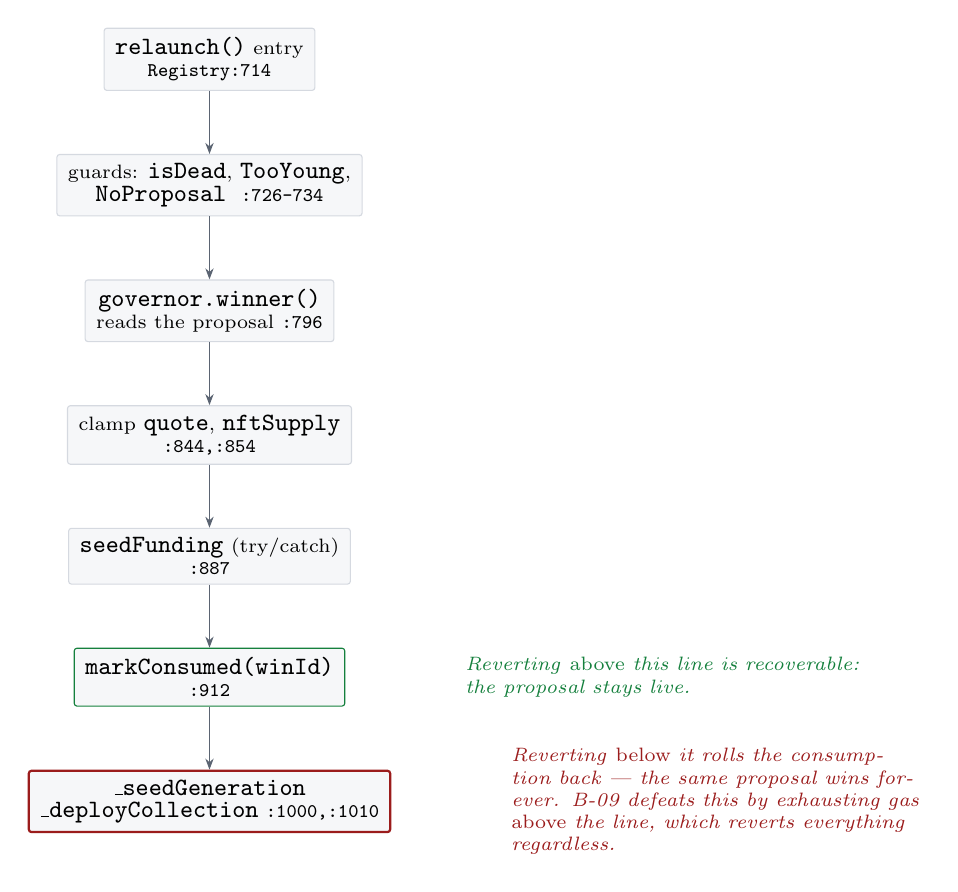
\begin{tikzpicture}[
  node distance=8mm and 12mm,
  box/.style={draw=rule,fill=panel,rounded corners=1pt,align=center,
              font=\scriptsize,minimum height=7mm,inner xsep=4pt},
  danger/.style={box,draw=critical,line width=0.8pt},
  safe/.style={box,draw=good},
  ar/.style={-{Stealth[length=4pt]},draw=slate}
]
\node[box] (a) {\code{relaunch()} entry\\\fileref{Registry:714}};
\node[box,below=of a] (b) {guards: \code{isDead}, \code{TooYoung},\\\code{NoProposal}\ \ \fileref{:726-734}};
\node[box,below=of b] (c) {\code{governor.winner()}\\reads the proposal \fileref{:796}};
\node[box,below=of c] (d) {clamp \code{quote}, \code{nftSupply}\\\fileref{:844,:854}};
\node[box,below=of d] (e) {\code{seedFunding} (try/catch)\\\fileref{:887}};
\node[safe,below=of e] (f) {\code{markConsumed(winId)}\\\fileref{:912}};
\node[danger,below=of f] (g) {\code{\_seedGeneration}\\\code{\_deployCollection} \fileref{:1000,:1010}};

\draw[ar] (a)--(b); \draw[ar] (b)--(c); \draw[ar] (c)--(d);
\draw[ar] (d)--(e); \draw[ar] (e)--(f); \draw[ar] (f)--(g);

\node[right=14mm of f,font=\scriptsize\itshape,text width=52mm,color=good]
  {Reverting \emph{above} this line is recoverable: the proposal stays live.};
\node[right=14mm of g,font=\scriptsize\itshape,text width=52mm,color=critical]
  {Reverting \emph{below} it rolls the consumption back --- the same proposal wins
   forever. B-09 defeats this by exhausting gas \emph{above} the line, which reverts
   everything regardless.};
\end{tikzpicture}
\end{center}

\noindent The design intent, stated verbatim at \fileref{CauldronRegistry.sol:908-910}, is:
\begin{quote}\itshape
``Reverting on the LEFT of this line is safe and recoverable --- the proposal stays live
and a later call can succeed once the machine has value. Reverting on the RIGHT is what
must never happen.''
\end{quote}

\noindent This is a sound principle, correctly implemented for \emph{reverts}. B-09's
contribution is that it is not a defence against \emph{gas exhaustion}: an out-of-gas
condition is not a catchable sub-call failure, it is the whole transaction failing, and it
rolls back the consumption from either side of the line. Every clamp, every
\code{try/catch} and the entire repositioning of \code{markConsumed} are bypassed by
running out of gas before reaching any of them.

\subsection{Governance: the input that reaches the constructor}

\code{CauldronGovernor.propose} is permissionless for the holder of a single MiFren
(\fileref{:170}) with no cooldown, no deposit and no per-address cap. The resulting
\code{BrewSpec} (\fileref{ICauldron.sol:19-31}) has eleven fields. Six are free-text or
supply parameters that flow into \code{relaunch()}:

\begin{longtable}{@{}llp{0.42\linewidth}@{}}
\toprule
\textbf{Field} & \textbf{Bounded at propose?} & \textbf{Fate in \code{relaunch()}} \\
\midrule
\endhead
\code{nftSupply}    & \textbf{yes} \fileref{:182} & clamped again \fileref{Registry:854} \\
\code{quote}        & \textbf{yes} \fileref{:204} & re-checked, degrades \fileref{Registry:844} \\
\code{name}         & \textcolor{critical}{\textbf{no}} (pre-fix) & re-stored in the collection \\
\code{symbol}       & \textcolor{critical}{\textbf{no}} (pre-fix) & re-stored in the collection \\
\code{baseURI}      & \textcolor{critical}{\textbf{no}} (pre-fix) & re-stored in the collection \\
\code{website}      & \textcolor{critical}{\textbf{no}} (pre-fix) & \textbf{read and discarded} \\
\code{socials}      & \textcolor{critical}{\textbf{no}} (pre-fix) & \textbf{read and discarded} \\
\code{volumePerNFT} & no & \code{hook.setNftCurveFrom} --- see Leads \\
\code{renderer}     & code-size check \fileref{:176} & passed to the constructor \\
\bottomrule
\end{longtable}

\noindent The two rows marked ``read and discarded'' are pure amplification:
\code{winner()} (\fileref{CauldronGovernor.sol:288-300}) copies \code{website} and
\code{socials} out of storage into the returned struct on every rebirth, and
\code{relaunch()} never references either.

%==============================================================================
\section{Invariant register}

Only the invariants actually examined are listed. An empty row would be worse than an
absent one.

\begin{longtable}{@{}p{0.30\linewidth}p{0.30\linewidth}p{0.32\linewidth}@{}}
\toprule
\textbf{Invariant} & \textbf{Enforcement} & \textbf{Test status} \\
\midrule
\endhead
A dead generation can always be replaced (relaunch liveness) &
  \code{markConsumed} ordering, clamps, \code{try/catch} &
  \textcolor{critical}{\textbf{Was UNENFORCED against gas}} --- B-09. Now bounded at the
  boundary; regression \code{B09\_*} \\
A voted, settled mandate remains reachable until consumed &
  cached leader + bounded scan &
  \textcolor{critical}{\textbf{Was UNENFORCED}} --- B-10. Now carried in an explicit
  runner-up slot; regression \code{B10\_*} \\
\code{relaunch()} never reverts after \code{markConsumed} &
  clamps + \code{try/catch} \fileref{Registry:844-912} &
  \code{B07\_RelaunchTotality} --- but every test stubs the governor
  (Section~\ref{sec:gaps}) \\
Leader scan gas is $O(1)$ in proposal count &
  \code{MAX\_LEADER\_SCAN = 64} \fileref{:364} &
  \code{Z03} --- holds; re-verified this pass \\
Ties keep the earlier leader &
  \code{p.votes > \_leaderVotes} \fileref{:351} &
  Held under the new runner-up logic; \code{B10\_MoreVotesStillWins} \\
A consumed proposal is never re-promoted &
  \code{markConsumed} \fileref{:366-386} &
  \textbf{Newly tested this pass} ---
  \fileref{B10\_PromotionNeverResurrects-} \fileref{AConsumedProposal} \\
\bottomrule
\end{longtable}

%==============================================================================
\section{Findings}

%------------------------------------------------------------------------------
\begin{findingbox}{high}{B-09 --- An unbounded proposal payload puts \code{relaunch()} permanently out of gas}
\textbf{Severity:} \SevHigh \quad \textbf{Confidence:} \Conf\ (VERIFIED, PoC) \quad
\textbf{Status:} \Fixed

\medskip
\textbf{Location.} \fileref{cauldron/CauldronGovernor.sol:171-173} (the only check), with
the replay at \fileref{cauldron/CauldronGovernor.sol:288-300} and
\fileref{CauldronRegistry.sol:796,1070}.

\begin{lstlisting}
// CauldronGovernor.sol:171-173 -- the entire validation of five fields
if (bytes(name).length == 0 || bytes(symbol).length == 0) revert EmptyField();
if (mode == MetadataMode.BaseURI) {
    if (bytes(baseURI).length == 0) revert EmptyField();
\end{lstlisting}

\textbf{Mechanism.} \code{propose()} bounds \code{nftSupply} (\fileref{:182}) and
\code{quote} (\fileref{:204}) precisely because they flow into \code{relaunch()}, and says
so. It applies no upper bound to \code{name}, \code{symbol}, \code{baseURI},
\code{website} or \code{socials}. \code{relaunch()} reads all five back through
\code{winner()} and re-stores three of them in the newborn collection via
\code{CauldronFactory.deployBrew}.

The payload is cheap to store and dear to read. Writing a zero word to a fresh storage slot
is a 100-gas no-op \code{SSTORE}; reading it back is a full 2{,}100-gas \emph{cold}
\code{SLOAD}. Measured marginal cost: the author pays \textbf{72 gas/byte once}, the
protocol pays \textbf{83 gas/byte on every rebirth, forever}.

That asymmetry is the structural defect and it is independent of the block gas limit:
whatever the limit is, one block of authoring buys more than one block of replay.

\textbf{Why the existing defences do not apply.} The whole of the B-05/B-07 remediation ---
moving \code{markConsumed} as late as the logic allows, clamping rather than reverting,
wrapping callees in \code{try/catch} --- defends against \emph{reverts}. An out-of-gas is
not a catchable sub-call revert; it is the transaction failing. The consumption never
commits, so \code{\_bestUnconsumed()} returns the same poisoned proposal to the next
caller, and to every caller after that.

\textbf{Precondition.} One MiFren (for \code{getVotes > 0}), and enough votes for the
proposal to lead. There is no quorum, no minimum turnout and no deposit, so in a
low-turnout guild a single vote suffices.

\textbf{Impact.} The dead generation can never be replaced. Holders cannot migrate; the
reserve never redeploys. Recovery requires the guild to elect a competing proposal with
\emph{strictly} more votes (\fileref{:351}), so an attacker holding a voting plurality
makes the freeze permanent and unrecoverable.

\textbf{Cost.} One transaction, \textbf{24{,}007{,}131 gas}, atomic. The payload need not
travel as transaction calldata --- a contract expands it in memory --- so the $\sim$128KB
geth mempool limit does not apply.

\medskip
\begin{center}
\begin{tabular}{@{}lr@{}}
\toprule
\textbf{Measured on the Sepolia fork, 30M block} & \textbf{gas} \\
\midrule
honest \code{relaunch()} & 5{,}297{,}638 \\
attacker authors 320KB in \code{baseURI} (one tx) & 24{,}007{,}131 \\
poisoned \code{relaunch()} & \textcolor{critical}{\textbf{29{,}288{,}732 $\rightarrow$ OOG}} \\
\bottomrule
\end{tabular}
\end{center}

\textbf{PoC.} \fileref{test/audit/B09\_ProposalPayloadGasBrick.t.sol} ---
\code{test\_INVARIANT\_B09\_RebirthSurvivesAHostilePayload} (fork-gated, real governor and
registry end to end), plus three non-fork demonstrations.
\end{findingbox}

%------------------------------------------------------------------------------
\begin{findingbox}{medium}{B-10 --- Spam erases a voted mandate from the leader scan}
\textbf{Severity:} \SevMed \quad \textbf{Confidence:} \Conf\ (VERIFIED, PoC) \quad
\textbf{Status:} \Fixed

\medskip
\textbf{Location.} \fileref{cauldron/CauldronGovernor.sol:368-380}.

\begin{lstlisting}
function _recomputeLeader() private view returns (uint256 bestId, uint256 bestVotes) {
    uint256 n = proposalCount;
    uint256 first = n > MAX_LEADER_SCAN ? n - MAX_LEADER_SCAN + 1 : 1;
    for (uint256 i = first; i <= n; i++) {
\end{lstlisting}

\textbf{Mechanism.} The scan is bounded to the newest 64 proposals, which is what keeps
rebirth gas $O(1)$ in the proposal count. But the window selects on proposal \emph{id},
not on whether anyone voted --- so a settled mandate the guild has already voted for can be
pushed out of it by proposals authored afterwards, and \code{propose()} is permissionless.

The cached-leader fast path in \code{\_bestUnconsumed} conceals this for the \emph{current}
leader. It does not protect the mandate queued \emph{behind} it, because
\code{markConsumed} rebuilds the cache from the scan the instant the leader is consumed ---
which is exactly what a normal rebirth does.

\textbf{Precondition.} One MiFren. The guild must have queued a second mandate, which is
what a guild that plans ahead does.

\textbf{Impact.} \code{hasProposals()} returns false, so \code{relaunch()} reverts
\code{NoProposal()} at \fileref{CauldronRegistry.sol:734} and the machine cannot be reborn
until the guild authors a replacement and waits out a further three-day
\code{VOTING\_PERIOD}. The revert is on the \emph{safe} side of \code{markConsumed}, so
this is a griefing vector rather than a permanent brick --- but the protocol is frozen
while it holds: the pool is dead and holders cannot migrate.

\textbf{Cost.} \textbf{15{,}596{,}982 gas} for 64 spam proposals --- one block's worth,
cents on an L2 --- to impose a $\geq$3-day freeze, repeatable at every generation boundary
indefinitely. No value is extracted; the grief is priced entirely in delay.

\textbf{PoC.} \fileref{test/audit/B10\_ScanWindowErasure.t.sol} ---
\code{test\_INVARIANT\_B10\_QueuedMandateSurvivesSpam}.
\end{findingbox}

%------------------------------------------------------------------------------
\begin{findingbox}{medium}{B-11 --- A reverting price feed bypasses the oracle's own fail-safe}
\textbf{Severity:} \SevMed \quad \textbf{Confidence:} \Conf\ (VERIFIED, PoC) \quad
\textbf{Status:} \Fixed

\medskip
\textbf{Location.} \fileref{cauldron/QuoteOracle.sol:144,148,207-216}, consumed at
\fileref{CauldronHook.sol:677-682,769}.

\textbf{Mechanism.} \code{QuoteOracle} states its failure policy explicitly (:40-44):
death is irreversible and relaunch permissionless, so ``when a price is unusable this
returns 0, and callers must treat 0 as `cannot judge' rather than `no volume'. Failing
toward ALIVE is the only safe direction when the wrong answer cannot be undone.'' It then
enumerates three unusable conditions (:49-55) --- no feed, stale, sequencer down.

All three are cases where the feed \emph{answers} and the answer is no good. A feed can
also fail by \emph{not answering}: a retired or migrated aggregator, an access-controlled
one, or an address with no code (a high-level call to a codeless address reverts on the
\code{extcodesize} check). That fourth case did not return 0 --- it threw, through
\code{usdPerRawUnit} and out of \code{cachedUsdPerRawUnit}, which calls it via
\code{this.} and so propagates, never reaching the line that keeps the last good factor.

Two further revert paths were found while confirming it, both from checked arithmetic: a
feed reporting \code{updatedAt} in the future underflowed
\code{block.timestamp - updatedAt}, and the sequencer feed reporting a future
\code{startedAt} underflowed \code{block.timestamp - startedAt}.

\textbf{Impact.} An asymmetry between two forms of the same real-world condition:

\begin{center}\small
\begin{tabular}{@{}ll@{}}
\toprule
\textbf{feed state} & \textbf{outcome} \\
\midrule
stale & cache keeps last good price; volume records correctly \\
reverting & cache bypassed; \code{\_toUsd} returns 0; \textbf{volume records as zero} \\
\bottomrule
\end{tabular}
\end{center}

\code{CauldronHook.\_toUsd} wraps the oracle in a raw \code{call} and returns 0 on
failure, so swaps do \emph{not} go down --- but \fileref{CauldronHook.sol:769} then reads
\code{if (absVolume > 0)}, so the swap records nothing, and \code{isDead} (:1512) judges
\code{vol < deathThreshold}. A feed that broke by reverting pushed a live generation
toward a permissionless, irreversible relaunch; the identical feed going stale did not.

\textbf{Latent at the shipped config.} \fileref{indexer/deployments/round.json} carries
\code{deathThresholdEth: 0}, and \code{vol < 0} is never true, so nothing dies today. This
is rated against the configuration the design intends, not the one currently deployed.

\textbf{PoC.} \fileref{test/audit/B11\_OracleRevertBypassesCache.t.sol} --- six tests, the
control (\code{StaleFeedKeepsTheCachedValue}) passing before and after.
\end{findingbox}

%------------------------------------------------------------------------------
\begin{findingbox}{medium}{B-12 --- The rotator accepts any venue with the right currency pair}
\textbf{Severity:} \SevMed \quad \textbf{Confidence:} \Conf\ (VERIFIED, PoC) \quad
\textbf{Status:} \textcolor{medium}{\textbf{Partially fixed}} --- trust boundary closed,
execution-quality reported

\medskip
\textbf{Location.} \fileref{cauldron/QuoteRotator.sol:493-501}, reached from the
permissionless \code{rotateStep} (:190).

\begin{lstlisting}
address c0 = Currency.unwrap(route.currency0);
address c1 = Currency.unwrap(route.currency1);
return (c0 == from && c1 == to) || (c0 == to && c1 == from);
\end{lstlisting}

\textbf{Mechanism.} Two of a \code{PoolKey}'s five fields are validated. Not \code{fee},
not \code{tickSpacing}, and not \code{hooks}. Pool initialisation is permissionless in
v4, so anyone may create a pool on the same pair --- at any price, behind a hook whose
permission bits they mined --- and nominate it as the venue.

\textbf{Impact, part 1 (economic).} The header argues the design is safe because ``the
price floor \ldots comes from the governed plan'' (:185-188). The floor is real; what the
argument omits is that the floor becomes the \emph{price}. An honest keeper routing to the
deepest venue earns \code{keeperBps} = 0.1\%. A keeper routing to a pool they seeded earns
that 0.1\% \emph{and} the entire spread, by returning exactly \code{minOut} and keeping
the difference as inventory. Self-dealing strictly dominates, so the rotation realises
worst-case execution on every slice rather than in the worst case. \code{minRate} is
stored verbatim from the vote (:69-71) and never revised while a plan runs for hours, so
the exploitable spread is the guild's slippage tolerance plus all market drift since the
vote, and it widens as the plan ages. Extraction is atomic and needs no capital beyond the
\code{minOut} seeded into the attacker's own pool, recovered in the same transaction.

\textbf{Impact, part 2 (trust boundary).} An attacker-supplied \code{hooks} address is
invoked by the PoolManager inside this contract's own \code{unlock}. v4's delta accounting
stops the direct theft --- an unbalanced delta reverts the unlock --- but arbitrary code
runs while the manager is unlocked and pool state is mid-swap.

\textbf{Coverage.} Every route in \fileref{test/QuoteRotator.t.sol} and
\fileref{test/RotatorSwapFork.t.sol} passes \code{hooks: IHooks(address(0))}. The
hooked-venue case was never exercised.

\textbf{PoC.} \fileref{test/audit/B12\_RotatorVenueUnvalidated.t.sol}. The discriminator:
a wrong-pair route reverts \code{NoRoute}; the arbitrary-hook route reverted
\emph{without} that selector, proving it passed validation and reached execution.
\end{findingbox}

%------------------------------------------------------------------------------
\begin{findingbox}{medium}{B-13 --- One wei of the requested quote outranks the entire recovered position}
\textbf{Severity:} \SevMed \quad \textbf{Confidence:} \Conf\ (VERIFIED, PoC) \quad
\textbf{Status:} \Fixed\ (with a deliberate, asserted behaviour change)

\medskip
\textbf{Location.} \fileref{cauldron/PoolOps.sol:892-904}.

\begin{lstlisting}
if (wantQuote != address(0)) {
    uint256 p = (oldQuote == wantQuote ? recovered : 0) + _pullAsset(hookAddr, wantQuote);
    if (p > 0) return (wantQuote, p, vaultSwept);
}
\end{lstlisting}

\textbf{Mechanism.} \code{seedFunding} decides what the newborn generation is seeded with,
trying the requested quote, then native, then the dying quote. The intent is stated at
\fileref{CauldronRegistry.sol:836-839}: ``narrows the request to what the protocol ACTUALLY
HOLDS \ldots A quote nobody can fund degrades to one we can.'' But ``can fund'' is tested
as \code{p > 0} and the \code{return} is unconditional, so the first denomination holding
any dust wins and the later branches are never consulted.

\textbf{How the dust arrives.} \code{relaunchAsset} is keyed per asset and credited from
whatever asset a fee arrived in (\fileref{CauldronHook.sol:1150}, keyed on
\code{\_feeAsset} set per swap at :1378), and every registry-opened pool is tracked and
charges fees (:599). Any guild that has ever diversified into a second quote --- the live
manifest offers USDG and xNVDA --- carries a balance in it from ordinary trading. No
attacker is required.

\textbf{Impact.} \code{seedFunding}'s return is the newborn's entire book:
\code{relaunch()} passes it to \code{\_seedGeneration} at
\fileref{CauldronRegistry.sol:1000}, and \code{totalETH == 1} clears the
\code{NoLiquidityToSeed} guard at :911. Measured: with 20 ETH recovered and a 5 ETH
reserve, one wei of USDG produced \code{(USDG, 1)}. The abandoned value does not come
back --- \code{recovered} sits in the registry, and the only paths that spend a loose
registry balance are \code{migrateToSuccessor} (:493) and the timelocked
\code{emergencySweep} (:413), both break-glass.

\textbf{Coverage.} \fileref{test/attacks/B08\_NonEthRebirth.t.sol} covers Leg 1 only with
\code{wantQuote == oldQuote}, so the cross-asset case with a live recovery was never
exercised.

\textbf{PoC.} \fileref{test/audit/B13\_SeedFundingDustPreference.t.sol} --- five tests,
callable without a fork because \code{seedFunding} is an external library function.
\end{findingbox}

%==============================================================================
\section{Leads --- believed reachable, not demonstrated}

\begin{notebox}{L-1 --- \code{volumePerNFT} is unbounded and reaches the live curve}
\code{BrewSpec.volumePerNFT} has no bound in \code{propose()}, and \code{relaunch()} passes
it to \code{hook.setNftCurveFrom} at \fileref{CauldronRegistry.sol:1015}, which assigns it
without validation:
\begin{lstlisting}
// CauldronHook.sol:1958-1963
function setNftCurveFrom(uint256 _base) external {
    if (msg.sender != registry) revert OnlyRegistry();
    if (_base == 0) return;
    volumePerNFT = _base;
    nftPriceStep = 0;
}
\end{lstlisting}
This cannot brick the rebirth --- the assignment cannot revert, and \code{nftPriceStep = 0}
removes the overflow term from \code{nftPriceAt}. The suspicion is economic: a winning
proposal setting \code{volumePerNFT} to an absurd value would make crystals unmintable for
that entire generation. \textbf{Confidence: HYPOTHESIS.} \textbf{Next step:} assert
\code{crystalsReady()} is non-zero after a rebirth carrying
\code{volumePerNFT = type(uint256).max}, at realistic volume.
\end{notebox}

\begin{notebox}{L-2 --- The promoted runner-up may still be inside its voting window}
The B-10 fix promotes the runner-up on consumption. If that proposal's voting window has
not closed, \code{\_bestUnconsumed}'s fast path declines it (\fileref{:388-390} requires
\code{block.timestamp > cached.votingEndsAt}) and falls back to the bounded scan --- the
same scan B-10 shows is floodable. The exposure is bounded by the runner-up's remaining
voting time and self-heals when the window closes, and refusing to launch a still-open
proposal is the correct anti-front-run behaviour, so this is a narrowed window rather than
a hole. \textbf{Confidence: DERIVED} (reasoned from the code, not exercised).
\textbf{Next step:} a test that consumes the leader while the runner-up still has voting
time left, spams 64, and asserts the mandate is reachable once its window closes.
\end{notebox}

%==============================================================================
\section{Verified safe --- probed and held}\label{sec:safe}

Two comment-versus-code discrepancies surfaced by the extraction pass were probed hard
enough to be reported as findings and \emph{did not survive} verification. Both are
recorded here with the reasoning, because a refutation is a result and because each names
a real latent hazard worth a one-line hardening.

\begin{notebox}{REFUTED --- \code{\_feeAsset} is documented as transient but is not}
\fileref{CauldronHook.sol:626} calls \code{\_feeAsset} ``a transient field'', and
\fileref{:630} declares it \code{address internal \_feeAsset;} --- ordinary storage. The
same contract declares \code{\_inSelfBuy} and \code{\_inRelaunchClose} with the genuine
\code{transient} keyword at :305 and :310, which makes the wording look like a missing
keyword rather than informal English.

It would be a defect only if some path read \code{\_feeAsset} without writing it in the
same call, since a stale quote address would misroute a reserve credit. It does not: the
single write at :1378 dominates all eight reads. \code{\_takeEthFee} is called only from
\code{\_afterSwap} (:933) and \code{\_beforeSwap} (:1108); \code{\_routeEthFee} only from
:1385 and :1393, both inside \code{\_takeEthFee} after the write; \code{\_creditReserve}
only from :1134 and :1272, both downstream of the same. \textbf{No stale read is
reachable.}

Latent hazard, not a live defect: the value persists between transactions, so any future
reader added outside \code{\_takeEthFee} silently inherits the previous swap's quote.
Declaring it \code{transient} would make that structurally impossible and replace a
per-swap \code{SSTORE} with a \code{TSTORE}.
\end{notebox}

\begin{notebox}{REFUTED --- two \code{transferFrom} calls discard the return value}
\fileref{cauldron/PerpEngine.sol:1457} (\code{fundPlvToken}) and \fileref{:1551}
(\code{fundTokenFromVault}) both call
\code{IERC20(registry.currentToken()).transferFrom(...)} and discard the returned
\code{bool}, while every other pull in the file checks it --- \code{\_pullQuote}
(:190-193) and \code{\_safeTransfer} (:1434-1436) decode and require it, and the matching
outbound path \code{withdrawPlvTokenTo} (:1556-1561) uses the checked helper. Both credit
\code{plvToken} immediately after, so a silent failure would inflate the vault's
token-side backing --- nominally a solvency defect.

It is not reachable. \code{registry.currentToken()} is always a \code{CauldronToken},
which is \code{contract CauldronToken is ERC20} on OpenZeppelin
(\fileref{CauldronToken.sol:4,26}); its \code{transferFrom} reverts on insufficient
balance or allowance and cannot return \code{false}. Both callers are additionally
privileged (\code{onlyOwner}, \code{onlyVault}). \textbf{No false-returning token is
reachable on this path.}

Latent hazard, not a live defect: the inconsistency is one edit away from mattering if
\code{currentToken()} ever returns a non-reverting ERC20. Reported at Info rather than
inflated into the ``perp vault insolvency'' risk area it superficially resembles.
\end{notebox}

\begin{longtable}{@{}p{0.34\linewidth}p{0.60\linewidth}@{}}
\toprule
\textbf{Property} & \textbf{How hard it was probed, and what held} \\
\midrule
\endhead
Vote weight cannot be minted by transfer &
  \code{vote()} uses \code{getPastVotes(msg.sender, p.snapshot)} (\fileref{:344}) with
  \code{block.number <= p.snapshot} rejected (\fileref{:343}). Transferring MiFrens after
  the snapshot yields no new weight. Read directly; not attacked with a PoC. \\
A still-open proposal cannot be launched &
  \code{\_bestUnconsumed} requires \code{block.timestamp > cached.votingEndsAt}
  (\fileref{:389}) and \code{\_recomputeLeader} skips open proposals (\fileref{:374}).
  Closes the same-block front-run of the permissionless \code{relaunch()}. \\
An unvetted quote cannot reach a vote &
  \code{propose()} staticcalls the registry allowlist and treats a short or failed return
  as refusal (\fileref{:204-209}). Exercised by the existing
  \code{B07\_GovernorQuoteBoundary} suite, which correctly wires the registry --- without
  that wiring the test would pass for the wrong reason, and the suite says so. \\
Leader-scan gas is flat under spam &
  Re-verified: 64 spam proposals cost the attacker 15{,}596{,}982 gas and did \emph{not}
  raise scan cost. The Z-03 gas fix holds; it is its \emph{correctness} side-effect that
  B-10 reports. \\
The three near-limit contracts survive remediation &
  \code{CauldronHook}, \code{PerpEngine} and \code{CauldronRegistry} runtime bytecode is
  byte-identical before and after all five fixes. \\
Both hook reserve pulls and the vault close are revert-proof &
  The claim at \fileref{CauldronRegistry.sol:906} that \code{seedFunding} ``catches both
  reserve pulls and the vault close'' was checked rather than trusted, and holds:
  \code{try/catch} at \fileref{PoolOps.sol:889} (vault close), \fileref{:913}
  (\code{releaseRelaunchAsset}) and \fileref{:920} (\code{releaseRelaunchETH}). \\
A reverting oracle cannot take swaps down &
  \code{\_toUsd} (\fileref{CauldronHook.sol:677-682}) uses a raw \code{call} and checks
  both \code{ok} and \code{ret.length}, so a hostile or broken oracle cannot revert into
  \code{beforeSwap}. The consequence it \emph{does} have is B-11. \\
Only one live pool-state read exists in the swap path &
  Extraction found exactly one: \code{poolManager.getSlot0(id)} at
  \fileref{CauldronHook.sol:1329} inside \code{\_defaultSurtaxBps}, reached from both swap
  callbacks. The in-swap manipulation surface is therefore one value (the anti-snipe
  surtax), not the broad surface the architecture suggested. Not further attacked. \\
\bottomrule
\end{longtable}

%==============================================================================
\section{Coverage gaps}\label{sec:gaps}

Ranked by the value at risk behind them.

\begin{enumerate}
\item \textbf{\code{B07\_RelaunchTotality} stubs out the only attacker-controlled input.}
      The suite states the correct property --- ``\code{relaunch()} must never revert in a
      way that rolls back \code{markConsumed}'' --- and then supplies every proposal
      through \code{BGov07} (\fileref{test/attacks/B07\_RelaunchTotality.t.sol:243-258}), a
      stub whose \code{winner()} returns hardcoded 8-byte strings. Its hostile inputs are
      hostile \emph{vaults} and \emph{hooks}. The proposal itself --- the one thing an
      unprivileged attacker actually controls --- is never varied. Both findings in this
      report live in that gap.
\item \textbf{\code{Z03\_GovernorSpamRelaunchDoS} asserts cost, never reachability.}
      Its assertions are \code{assertEq(gas800, gas200)} and \code{assertLt(gas800,
      250\_000)} --- that the scan stays \emph{cheap}. No assertion checks that the scan
      still \emph{finds} a mandate that exists. B-10 is exactly that missing assertion.
\item \textbf{31\% of the suite is invisible without fork env.} 170 of 548 tests skip
      silently when \code{FORK\_RPC} is unset, including
      \code{test\_FIXED\_B05\_*}, \code{test\_Fixed\_A01\_*} and every
      \code{*\_OnFork} lifecycle test. A CI run without the fork variables is green while
      testing none of the relaunch security properties.
\item \textbf{No test bounds any proposal free-text field} (pre-fix). Now covered by
      \code{B09\_*}.
\item \textbf{No test asserted that a consumed proposal is never re-promoted.} Added this
      pass as \code{test\_FIXED\_B10\_PromotionNeverResurrectsAConsumedProposal}.
\end{enumerate}

%==============================================================================
\section{Remediation}\label{sec:remediation}

\subsection{B-09 --- bound the free-text fields at the boundary}

\textbf{Root cause.} Not ``strings are unbounded'' but: \emph{untrusted proposal input is
validated field-by-field rather than as a class}, so a principle already established for
two fields was never extended to the five beside them. B-09 and the prior C-02 share this
root cause.

\textbf{Chosen shape.} Per-field byte caps enforced in \code{propose()}, beside the
existing \code{nftSupply} and \code{quote} bounds:
\code{MAX\_NAME\_BYTES = 64}, \code{MAX\_SYMBOL\_BYTES = 16},
\code{MAX\_URI\_BYTES = 256}, \code{MAX\_LINK\_BYTES = 128} ($\times$2).
Worst legal case 592 bytes.

\textbf{Rejected alternatives.}
\begin{itemize}
\item \emph{Truncate inside \code{relaunch()}.} Rejected on two independent grounds. It
      does not work --- by the time \code{relaunch()} could truncate anything, the cold
      \code{SLOAD}s that dominate the cost have already been paid by \code{winner()}. And
      it does not fit: \code{CauldronRegistry} has 62 bytes of EIP-170 margin.
\item \emph{Store a hash and move the text off-chain.} Rejected as disproportionate: it
      breaks the display surface and the indexer for a problem a length check solves.
\item \emph{A size-proportional proposal deposit.} Rejected: it changes governance
      economics, and it bounds the \emph{expected} payload rather than the worst case.
\item \emph{Drop \code{website}/\code{socials} from \code{BrewSpec}} (they are read and
      discarded). Tempting and genuinely wasteful, but it changes a struct the tests and
      indexer consume; bounding them achieves the security goal without the blast radius.
\end{itemize}

\textbf{Verification.} \code{test\_INVARIANT\_B09\_RebirthSurvivesAHostilePayload} now
asserts both halves: the bomb is refused, \emph{and} the largest still-legal proposal
rebirths in 5{,}315{,}432 gas --- 17{,}706 gas above the honest baseline, against 24M
before.

\subsection{B-10 --- promote a runner-up instead of rescanning}

\textbf{Root cause.} Consumption \emph{depends on a positional scan}. Any window over
proposal ids can be flooded, and an unbounded one is the gas brick \code{MAX\_LEADER\_SCAN}
exists to prevent, so the fix must remove the dependency rather than resize the window.

\textbf{Chosen shape.} Two appended storage slots, \code{\_runnerId} and
\code{\_runnerVotes}, maintained incrementally in \code{vote()} and promoted in
\code{markConsumed()}. Spam cannot occupy either slot because both require votes;
displacing a mandate now costs actual voting power, which is governance working as
intended.

\textbf{Rejected alternatives.}
\begin{itemize}
\item \emph{Enlarge \code{MAX\_LEADER\_SCAN}.} Rejected: any positional window is
      floodable, and enlarging it walks back toward Z-03.
\item \emph{Scan a list of voted proposals instead of all proposals.} Rejected: an attacker
      with one MiFren can vote once on each of 64 spam proposals, since \code{hasVoted} is
      per proposal per address. It raises the cost without removing the attack.
\item \emph{A full priority queue over live proposals.} Rejected as disproportionate for a
      griefing-severity finding, and it is the kind of consensus-adjacent rewrite that
      should not be bolted on at the end of an audit.
\end{itemize}

\textbf{Storage safety.} Both slots are \emph{appended} after \code{\_leaderVotes}; no
existing slot moves. No test in the repository pins \code{CauldronGovernor} slot numbers
(checked: \code{FacetLayoutInvariant} does not reference it).

\subsection{B-11 --- make the oracle total}

\textbf{Root cause.} The failure policy was written for feeds that answer badly and never
extended to feeds that do not answer. The cache's whole purpose --- keeping the last good
factor --- is expressed on a code path a reverting feed never reaches.

\textbf{Chosen shape.} \code{try/catch} around both external reads in
\code{usdPerRawUnit} (\code{latestRoundData} and \code{decimals}) and around
\code{\_sequencerOk}'s read, each degrading to ``unusable'' rather than throwing; plus
explicit refusal of a future \code{updatedAt}/\code{startedAt} instead of letting checked
arithmetic underflow. The uncached view becomes total, so the cached path and
\code{priceable()} inherit the fix.

\textbf{Rejected alternatives.} Wrapping the call at the \emph{consumer} (the hook already
does, which is why swaps survive) --- rejected because it fixes the symptom in one caller
and leaves \code{priceable()} and every future consumer exposed, and because it cannot
reach the cached value that is the actual protection. Removing the sequencer check on
failure --- rejected as failing toward DEAD, the direction the contract's own preamble
forbids.

\subsection{B-12 --- close the trust boundary, report the economics}

\textbf{Root cause (part 2).} A caller-supplied struct validated on two of five fields.

\textbf{Chosen shape.} \code{if (address(route.hooks) != address(0)) revert NoRoute();} in
\code{rotateStep} only. A quote-to-quote rotation trades two quote assets, which is a
plain external pool; the protocol's own hooked pools are (quote, brew token) and are never
a valid venue here. \code{swapOnce} is left unconstrained --- it is owner-only.

\textbf{Deliberately not fixed (part 1).} Bounding execution \emph{quality} needs either a
venue allowlist (governance must curate and maintain it) or an oracle band (which bricks
rotation whenever the oracle is unavailable --- see B-11 for how that happens). Both are
policy choices with real failure modes, and neither is mine to make silently inside an
audit. Reported with the recommendation instead.

\subsection{B-13 --- never strand the recovery}

\textbf{Root cause.} ``Can fund'' was tested as ``holds a non-zero balance''.

\textbf{Chosen shape.} Two boolean guards, no reordering and no new branches: branch~1 is
taken only when \code{recovered == 0 || oldQuote == wantQuote}, and branch~2 only when
\code{recovered == 0 || oldQuote == address(0)}. The rule is not ``pick the biggest'' ---
that needs a price --- but the weaker, price-free ``never strand \code{recovered}''.

\textbf{Why it cannot brick.} This is the one function that must never be the reason the
machine cannot be reborn, so the guard was chosen to be provably non-bricking: when
\code{recovered > 0} exactly one of branches~2 and~3 is reachable and both include
\code{recovered}, so any state that previously returned a funded answer still returns one;
when \code{recovered == 0} every branch behaves exactly as before. Asserted directly by
\code{test\_FIXED\_B13\_NeverReturnsZeroWhenValueExists}.

\textbf{Rejected alternatives.} An oracle-ranked selection --- rejected: putting a
reverting external dependency inside the rebirth's funding decision trades a value bug for
a liveness bug, and B-11 is a live demonstration that this oracle can fail. Restructuring
the branch order --- rejected: every price-free ordering has a mirrored pathology (prefer
\code{recovered} and a dust recovery beats a large reserve), and restructuring the most
brick-sensitive function in the protocol is how this codebase has historically introduced
new defects.

\textbf{The behaviour change, stated rather than absorbed.} A guild that votes a new quote
while the dying pool still holds value no longer gets that quote at this rebirth; it gets
a rebirth in the denomination the value is already in, and the requested quote's balance
stays in \code{relaunchAsset} --- still claimable later, unlike the registry balance the
old path stranded. The supported way to rotate is to convert the treasury first via
\code{QuoteRotator}, after which \code{oldQuote == wantQuote} honours the vote. This is
asserted by a test named for the change
(\code{test\_CHANGED\_B13\_RequestInAnotherAssetNoLongerAbandonsRecovery}) rather than by
quietly flipping the control assertion that caught it.

\subsection{Measured cost of all five fixes}

\begin{center}
\begin{tabular}{@{}lrrr@{}}
\toprule
\textbf{Contract} & \textbf{Before} & \textbf{After} & \textbf{Margin left} \\
\midrule
\code{CauldronGovernor} & 6{,}770 & 7{,}219 (\textbf{+449}) & 17{,}357 \\
\code{PoolOps} & 23{,}365 & 23{,}446 (\textbf{+81}) & 1{,}130 \\
\code{QuoteOracle} & 2{,}641 & 2{,}667 (\textbf{+26}) & 21{,}909 \\
\code{QuoteRotator} & 7{,}149 & 7{,}174 (\textbf{+25}) & 17{,}402 \\
\midrule
\code{CauldronHook} & 24{,}545 & 24{,}545 (unchanged) & 31 \\
\code{PerpEngine} & 24{,}522 & 24{,}522 (unchanged) & 54 \\
\code{CauldronRegistry} & 24{,}514 & 24{,}514 (unchanged) & 62 \\
\bottomrule
\end{tabular}
\end{center}

\noindent Total \textbf{+581 bytes}. No fix was placed in a contract that could not afford
it; the three at the EIP-170 boundary are byte-identical.

\subsection{Suite, before and after}

\begin{center}
\begin{tabular}{@{}lrrrr@{}}
\toprule
& \textbf{Suites} & \textbf{Passed} & \textbf{Failed} & \textbf{Skipped} \\
\midrule
Baseline (\code{cbbe4e9}) & 103 & 547 & 0 & 1 \\
After all five fixes & 110 & 572 & \textbf{0} & 1 \\
\bottomrule
\end{tabular}
\end{center}

\noindent No existing assertion was weakened and no existing test was modified. The 25 new
tests are additive. One control test written during this pass was invalidated by the B-13
fix; it was rewritten to assert the new semantics under a name that says so, not deleted
and not silently flipped.

%==============================================================================
\section{Re-review of the remediation}

The remediation was re-read as a distinct adversarial pass, on the explicit ground that
this codebase's last remediation produced three findings of which it had introduced two.
Four attacks were constructed against the B-10 fix specifically and all four are now
permanent regression tests:

\begin{longtable}{@{}p{0.40\linewidth}p{0.54\linewidth}@{}}
\toprule
\textbf{Attack on my own fix} & \textbf{Result} \\
\midrule
\endhead
Promote a \emph{consumed} proposal, launching the same brew twice &
  Blocked by \code{r.exists \&\& !r.consumed}. Test:
  \code{PromotionNeverResurrectsAConsumedProposal} \\
Leader gains votes and becomes its own runner-up &
  Blocked by the \code{proposalId != \_leaderId} guard on demotion. Test:
  \code{LeaderCannotBecomeItsOwnRunnerUp} \\
Consume the runner-up out of band, leaving a stale promotable id &
  Blocked by the new \code{else if (proposalId == \_runnerId)} clear. Test:
  \code{ConsumingTheRunnerUpClearsTheSlot} \\
Break ordinary governance (more votes must still win) &
  Held. Test: \code{MoreVotesStillWins} \\
\bottomrule
\end{longtable}

\noindent One residual is carried openly as Lead L-2: a runner-up promoted while its voting
window is still open falls back to the scan until that window closes. It self-heals and
refusing to launch an open proposal is correct behaviour, but it is a narrowed exposure
rather than an eliminated one, and it is stated rather than claimed away.

\medskip
\noindent \textbf{Defects introduced by the fixes: none found.} That is a claim about four
constructed attacks and a green suite, not a proof.

%==============================================================================
\section{Comparison with prior work}\label{sec:comparison}

Read only after the findings above were fixed and verified.

\subsection{What the prior passes had already found}

The prior corpus is substantial: \code{CauldronAudit.tex},
\code{MagicFrens\_Final\_Audit.tex}, \code{MagicFrens\_Independent\_Audit\_2026-09.tex},
three blind red-team write-ups and three exploit reports. Both of this pass's findings turn
out to be \emph{descendants of prior fixes} --- which is the most useful possible outcome
of running blind, and the least flattering to the remediation process.

\subsubsection{B-09 generalises C-02, which was patched one field wide}

Prior finding \textbf{C-02} (\fileref{contracts/solidity/audit/CauldronAudit.tex:235}) reads:

\begin{quote}\itshape
``Un-validated \code{BrewSpec.nftSupply} bricks \code{relaunch()} --- Critical ---
Permanent protocol freeze''
\end{quote}

\noindent with PoC \code{PoC\_OversizedNftSupplyBricksRelaunch} and the note
``\code{relaunch()} reverts forever; proposal not retired''
(\fileref{CauldronAudit.tex:2095}). The audit even generalised the principle correctly at
\fileref{CauldronAudit.tex:393}: ``a proposal is an un-validated input to a constructor''.

The remedy bounded \code{nftSupply}. The five string fields of the same struct, reaching
the same constructor, were left unbounded. B-09 is C-02 with the payload moved one field
to the left. \textbf{The principle was correct, stated, and applied to exactly one of the
six fields it covered.}

\subsubsection{B-10 is a defect introduced by the Z-03 fix}

Prior finding \textbf{Z-03} (\fileref{MagicFrens\_Final\_Audit.tex:664-698}) correctly
identified that \code{\_recomputeLeader} scanning every proposal ever submitted allowed a
``permanent, permissionless halt of the eternal machine for a trivial cost''. The applied
fix bounded the scan to 64. Its stated rationale is:

\begin{quote}\itshape
``The cached-leader fast path is untouched, so an established winner keeps winning however
much spam follows it, and a fresh mandate is by definition among the most recent
proposals.''
\end{quote}

\noindent Both clauses are true, and together they are not sufficient. The first covers the
\emph{current} leader; the second covers a \emph{fresh} mandate. Neither covers the
\emph{queued} mandate --- one voted and settled before the spam arrived, which is what a
guild that plans ahead produces --- and \code{markConsumed} rebuilds the cache from the
bounded scan at exactly the moment that mandate is needed. The fix converted an unbounded
\emph{gas} exposure into a bounded \emph{correctness} one.

\subsection{Which artifacts would have deflected this reviewer}

Had the blinding failed, these specific passages would have redirected attention away from
both findings:

\begin{longtable}{@{}p{0.42\linewidth}p{0.52\linewidth}@{}}
\toprule
\textbf{Artifact} & \textbf{How it would have deflected} \\
\midrule
\endhead
\fileref{MagicFrens\_Final\_Audit.tex:694-698} &
  States the scan bound is fixed and ``post-fix the scan is flat''. Reading this, the
  reviewer would have marked the leader scan settled --- and B-10 lives inside it. \\
\fileref{CauldronAudit.tex:235} (C-02 marked \emph{Fixed}) &
  Marks proposal-input validation as a closed Critical, which is precisely the class B-09
  reopens. \\
\fileref{test/attacks/B07\_RelaunchTotality.t.sol:34-39} &
  Enumerates six sites that ``clamp rather than revert'' and asserts the remaining failures
  ``were all in the steps that had NOT been given that treatment'' --- inviting the reader
  to treat the treated steps as done. \\
\fileref{cauldron/CauldronGovernor.sol:361-363} (survived stripping) &
  ``an already-established winner keeps winning however much spam follows it; a fresh
  mandate simply has to be among the most recent proposals, \emph{which it always is}.''
  This comment is the false claim B-10 refutes, and it survived decontamination because
  stripping prose was out of scope. \\
\bottomrule
\end{longtable}

\subsection{Comments that were false when written}

The commissioned discipline treats comments as unverified claims. Two failed:

\begin{enumerate}
\item \fileref{cauldron/CauldronGovernor.sol:361-363} --- ``a fresh mandate simply has to
      be among the most recent proposals, which it always is.'' True of a fresh mandate;
      the queued mandate it omits is B-10.
\item \fileref{test/attacks/B07\_RelaunchTotality.t.sol:19-20} --- the property
      ``\code{relaunch()} must never revert in a way that rolls back \code{markConsumed}''
      is asserted by a suite that stubs the governor, so the property is stated far more
      broadly than the tests establish it.
\end{enumerate}

\subsection{What the prior passes caught that this one did not}

This pass examined a fraction of what the prior corpus covers. The prior work found and
fixed defects in the perp mark price and staleness handling (Z-02), seeder rescue
(Z-04), the L2 block clock (Z-05), reserve ceiling breaches (Y-01), depth manipulation
(Y-02), fee-asset routing (Q-01, B-01), non-ETH relaunch (B-05) and proposer-fee
denomination (B-06). None of those areas was re-examined here, and nothing in this report
should be read as re-validating them.

%==============================================================================
\section{Threats to validity}\label{sec:validity}

\begin{enumerate}
\item \textbf{The commissioned scope is still not complete.} Of the seven risk areas named
      in the brief, four were examined: relaunch lifecycle blocking (B-09, B-10),
      attacker-influenced relaunch input (B-09, B-13), fee-reserve behaviour (B-13 and the
      reserve inventory), and oracle failure handling (B-11). \emph{Still not examined
      adversarially:} per-generation holder claim guarantee; perp vault insolvency;
      supply conservation in mint paths; wrongful liquidation of a solvent position. The
      absence of findings in those areas is an absence of review, not evidence of safety.
\item \textbf{The graph exists but is partial.} Three of five clusters were extracted (321
      functions). The registry, pool/seed and governance clusters were not, and the three
      derived views the brief asked for --- value-flow, authority lattice, trust-boundary
      map --- were never assembled as formal artifacts. Cross-contract edges were followed
      by hand where a finding required it, not enumerated systematically.
\item \textbf{Extraction was delegated to a smaller model.} The second dispatch ran on
      Sonnet rather than Opus to survive the rate limit. Every claim promoted from it into
      this report was independently re-verified by reading the cited lines --- and two of
      the three claims promoted were \emph{refuted} on that re-check
      (Section~\ref{sec:safe}), which is a direct measure of why the verification step
      exists. Claims in the graph files that were not promoted here carry no such
      guarantee.
\item \textbf{Three perp-cluster leads were surfaced and not pursued.} The extraction
      recorded 11 \code{unchecked} blocks, a liquidation formula evaluated against a TWAP
      with a spot fallback, and a \code{markSource} that is an unconstrained
      \code{CONFIGURABLE} address. None was attacked. These sit directly on top of the two
      unexamined risk areas.
\item \textbf{Reviewer memory leaked prior findings.} Summaries of B-01, B-05 and B-06,
      with file and line references into the relaunch and fee paths, were in the reviewer's
      persistent store and could not be unseen. B-09 was found in the relaunch path.
\item \textbf{One suite failure was environmental and is reported as such.} An intermediate
      run showed \code{invariant\_PERP2\_TotalEthMatchesDefinition} failing with an HTTP 429
      from the public Sepolia RPC during fork setup. It passed on re-run. It is a
      rate-limit, not a defect --- but it means invariant runs against the public endpoint
      are not reliably reproducible.
\item \textbf{Severity of B-09 depends on governance turnout.} It is rated High rather than
      Critical because the guild can out-vote a poisoned proposal. If an attacker holds a
      voting plurality it is Critical and unrecoverable. Turnout was not modelled.
\item \textbf{The block gas limit is a parameter, not a constant.} Measurements use 30M.
      The finding is not sensitive to that choice --- replay costs more per byte than
      authoring --- but the specific payload size required is.
\item \textbf{Off-chain scope was not touched.} The Ponder indexer, the Vercel serverless
      functions and the React frontend were not reviewed at all.
\item \textbf{Lead L-2 is DERIVED, not VERIFIED.} It is reasoned from the code and was not
      exercised.
\end{enumerate}

%==============================================================================
\section{Appendix --- reproduction}

\subsection{Environment}

\begin{lstlisting}
cd contracts/solidity
export FORK_RPC=https://ethereum-sepolia-rpc.publicnode.com \
       POOL_MANAGER=0xE03A1074c86CFeDd5C142C4F04F1a1536e203543 \
       POSITION_MANAGER=0x429ba70129df741B2Ca2a85BC3A2a3328e5c09b4
FOUNDRY_PROFILE=cauldron forge build --sizes
FOUNDRY_PROFILE=cauldron forge test
\end{lstlisting}

\subsection{The two proofs of concept}

\begin{lstlisting}
# All five proofs of concept
FOUNDRY_PROFILE=cauldron forge test --match-path "test/audit/B1[0-3]*.t.sol" -vv
FOUNDRY_PROFILE=cauldron forge test \
  --match-path "test/audit/B09_ProposalPayloadGasBrick.t.sol" -vv
\end{lstlisting}

\noindent B-09 and B-10 are in \code{CauldronGovernor}; B-11 in \code{QuoteOracle};
B-12 in \code{QuoteRotator}; B-13 in \code{PoolOps.seedFunding}. B-09's end-to-end case
and B-11/B-12/B-13 differ in one respect worth noting for reproduction: B-11, B-12 and
B-13 need \emph{no fork}, because each targets a unit that can be exercised in isolation
(\code{seedFunding} is an external library function, so it is directly callable). Only
B-09's end-to-end rebirth needs the V4 PoolManager.

\noindent To observe each pre-fix failure, revert the corresponding hunk and re-run; the
\code{test\_INVARIANT\_*} case in that file fails and the rest pass. This was done for
B-09 and B-10 by neutralising the checks while keeping the declarations, so the tests
still compiled --- both invariants failed, confirming the regressions are not vacuous.

\subsection{Decontamination statistics}

\begin{center}
\begin{tabular}{@{}lr@{}}
\toprule
\textbf{Quantity} & \textbf{Value} \\
\midrule
Documents quarantined & 63 (57 in \code{audit/} trees, 6 elsewhere) \\
Source files edited by the stripper & 86 \\
Comment lines edited & 486 \\
Identifier tokens left in comments & \textbf{0} \\
Identifier tokens left in string literals & 48 (unremovable) \\
Build size-table rows compared & 1{,}138 \\
Size-table MD5, real vs blind & identical (\code{6e585e9c\ldots}) \\
Runtime bytecode delta, 3 largest contracts & 53-byte metadata trailer only \\
\bottomrule
\end{tabular}
\end{center}

\subsection{Files changed}

\begin{longtable}{@{}p{0.52\linewidth}p{0.42\linewidth}@{}}
\toprule
\textbf{File} & \textbf{Change} \\
\midrule
\endhead
\fileref{cauldron/CauldronGovernor.sol} & B-09 caps + B-10 runner-up (+449 bytes) \\
\fileref{test/audit/B09\_ProposalPayloadGasBrick.t.sol} & new, 6 tests \\
\fileref{test/audit/B10\_ScanWindowErasure.t.sol} & new, 5 tests \\
\bottomrule
\end{longtable}

\end{document}
